\documentclass[]{article}
\usepackage{lmodern}
\usepackage{amssymb,amsmath}
\usepackage{ifxetex,ifluatex}
\usepackage{fixltx2e} % provides \textsubscript
\ifnum 0\ifxetex 1\fi\ifluatex 1\fi=0 % if pdftex
  \usepackage[T1]{fontenc}
  \usepackage[utf8]{inputenc}
\else % if luatex or xelatex
  \ifxetex
    \usepackage{mathspec}
  \else
    \usepackage{fontspec}
  \fi
  \defaultfontfeatures{Ligatures=TeX,Scale=MatchLowercase}
\fi
% use upquote if available, for straight quotes in verbatim environments
\IfFileExists{upquote.sty}{\usepackage{upquote}}{}
% use microtype if available
\IfFileExists{microtype.sty}{%
\usepackage{microtype}
\UseMicrotypeSet[protrusion]{basicmath} % disable protrusion for tt fonts
}{}
\usepackage[margin=1in]{geometry}
\usepackage{hyperref}
\hypersetup{unicode=true,
            pdftitle={naniar: Expanding ggplot2 to better visual exploration missingsness},
            pdfauthor={Nicholas Tierney},
            pdfborder={0 0 0},
            breaklinks=true}
\urlstyle{same}  % don't use monospace font for urls
\usepackage{color}
\usepackage{fancyvrb}
\newcommand{\VerbBar}{|}
\newcommand{\VERB}{\Verb[commandchars=\\\{\}]}
\DefineVerbatimEnvironment{Highlighting}{Verbatim}{commandchars=\\\{\}}
% Add ',fontsize=\small' for more characters per line
\usepackage{framed}
\definecolor{shadecolor}{RGB}{248,248,248}
\newenvironment{Shaded}{\begin{snugshade}}{\end{snugshade}}
\newcommand{\KeywordTok}[1]{\textcolor[rgb]{0.13,0.29,0.53}{\textbf{{#1}}}}
\newcommand{\DataTypeTok}[1]{\textcolor[rgb]{0.13,0.29,0.53}{{#1}}}
\newcommand{\DecValTok}[1]{\textcolor[rgb]{0.00,0.00,0.81}{{#1}}}
\newcommand{\BaseNTok}[1]{\textcolor[rgb]{0.00,0.00,0.81}{{#1}}}
\newcommand{\FloatTok}[1]{\textcolor[rgb]{0.00,0.00,0.81}{{#1}}}
\newcommand{\ConstantTok}[1]{\textcolor[rgb]{0.00,0.00,0.00}{{#1}}}
\newcommand{\CharTok}[1]{\textcolor[rgb]{0.31,0.60,0.02}{{#1}}}
\newcommand{\SpecialCharTok}[1]{\textcolor[rgb]{0.00,0.00,0.00}{{#1}}}
\newcommand{\StringTok}[1]{\textcolor[rgb]{0.31,0.60,0.02}{{#1}}}
\newcommand{\VerbatimStringTok}[1]{\textcolor[rgb]{0.31,0.60,0.02}{{#1}}}
\newcommand{\SpecialStringTok}[1]{\textcolor[rgb]{0.31,0.60,0.02}{{#1}}}
\newcommand{\ImportTok}[1]{{#1}}
\newcommand{\CommentTok}[1]{\textcolor[rgb]{0.56,0.35,0.01}{\textit{{#1}}}}
\newcommand{\DocumentationTok}[1]{\textcolor[rgb]{0.56,0.35,0.01}{\textbf{\textit{{#1}}}}}
\newcommand{\AnnotationTok}[1]{\textcolor[rgb]{0.56,0.35,0.01}{\textbf{\textit{{#1}}}}}
\newcommand{\CommentVarTok}[1]{\textcolor[rgb]{0.56,0.35,0.01}{\textbf{\textit{{#1}}}}}
\newcommand{\OtherTok}[1]{\textcolor[rgb]{0.56,0.35,0.01}{{#1}}}
\newcommand{\FunctionTok}[1]{\textcolor[rgb]{0.00,0.00,0.00}{{#1}}}
\newcommand{\VariableTok}[1]{\textcolor[rgb]{0.00,0.00,0.00}{{#1}}}
\newcommand{\ControlFlowTok}[1]{\textcolor[rgb]{0.13,0.29,0.53}{\textbf{{#1}}}}
\newcommand{\OperatorTok}[1]{\textcolor[rgb]{0.81,0.36,0.00}{\textbf{{#1}}}}
\newcommand{\BuiltInTok}[1]{{#1}}
\newcommand{\ExtensionTok}[1]{{#1}}
\newcommand{\PreprocessorTok}[1]{\textcolor[rgb]{0.56,0.35,0.01}{\textit{{#1}}}}
\newcommand{\AttributeTok}[1]{\textcolor[rgb]{0.77,0.63,0.00}{{#1}}}
\newcommand{\RegionMarkerTok}[1]{{#1}}
\newcommand{\InformationTok}[1]{\textcolor[rgb]{0.56,0.35,0.01}{\textbf{\textit{{#1}}}}}
\newcommand{\WarningTok}[1]{\textcolor[rgb]{0.56,0.35,0.01}{\textbf{\textit{{#1}}}}}
\newcommand{\AlertTok}[1]{\textcolor[rgb]{0.94,0.16,0.16}{{#1}}}
\newcommand{\ErrorTok}[1]{\textcolor[rgb]{0.64,0.00,0.00}{\textbf{{#1}}}}
\newcommand{\NormalTok}[1]{{#1}}
\usepackage{graphicx,grffile}
\makeatletter
\def\maxwidth{\ifdim\Gin@nat@width>\linewidth\linewidth\else\Gin@nat@width\fi}
\def\maxheight{\ifdim\Gin@nat@height>\textheight\textheight\else\Gin@nat@height\fi}
\makeatother
% Scale images if necessary, so that they will not overflow the page
% margins by default, and it is still possible to overwrite the defaults
% using explicit options in \includegraphics[width, height, ...]{}
\setkeys{Gin}{width=\maxwidth,height=\maxheight,keepaspectratio}
\IfFileExists{parskip.sty}{%
\usepackage{parskip}
}{% else
\setlength{\parindent}{0pt}
\setlength{\parskip}{6pt plus 2pt minus 1pt}
}
\setlength{\emergencystretch}{3em}  % prevent overfull lines
\providecommand{\tightlist}{%
  \setlength{\itemsep}{0pt}\setlength{\parskip}{0pt}}
\setcounter{secnumdepth}{0}
% Redefines (sub)paragraphs to behave more like sections
\ifx\paragraph\undefined\else
\let\oldparagraph\paragraph
\renewcommand{\paragraph}[1]{\oldparagraph{#1}\mbox{}}
\fi
\ifx\subparagraph\undefined\else
\let\oldsubparagraph\subparagraph
\renewcommand{\subparagraph}[1]{\oldsubparagraph{#1}\mbox{}}
\fi

%%% Use protect on footnotes to avoid problems with footnotes in titles
\let\rmarkdownfootnote\footnote%
\def\footnote{\protect\rmarkdownfootnote}

%%% Change title format to be more compact
\usepackage{titling}

% Create subtitle command for use in maketitle
\newcommand{\subtitle}[1]{
  \posttitle{
    \begin{center}\large#1\end{center}
    }
}

\setlength{\droptitle}{-2em}
  \title{naniar: Expanding ggplot2 to better visual exploration missingsness}
  \pretitle{\vspace{\droptitle}\centering\huge}
  \posttitle{\par}
  \author{Nicholas Tierney}
  \preauthor{\centering\large\emph}
  \postauthor{\par}
  \predate{\centering\large\emph}
  \postdate{\par}
  \date{14/12/2016}


\begin{document}
\maketitle

\section{Introduction}\label{introduction}

Missing data is ubiquitous in data analysis, and are often the source of
much energy, frustration, and confusion. Since 2014 there has been
substantial development in the area of ``tidy data'' (@wickham), which
states the (surprisingly simple!) rule that each row is an observation
and each column is a variable, which makes it easy to reason with data.
This paper describes approaches for summarising missing data in
numerical and graphical forms whilst maintaining a tidy format.

\section{Types of missing data}\label{types-of-missing-data}

Canonical sources of missing data are questionnaires. Data obtained from
questionnaires are often subject to both unknown and known missingness
structure. For example, unknown missing data structure can arise from
respondents accidentally failing to answer questions or inadvertently
providing inappropriate answers. Known missing data structure data may
arise due to the structure of the questionnaire. For example, the first
question on a survey might be: `If YES, skip to question 4', resulting
in questions 2 and 3 missing. If the structure of the questionnaire is
known, this type of missingness can be evaluated easily. However, if
this information is not available, the mechanism responsible for
producing missing data must be inferred from the data.

Another common source of known and unknown structured missingness is
medical examination data. The results of particular medical tests may
be: missing for purely random reasons, missing due to the procedure, or
missing based on decisions arising from the observed data. For example,
a young patient is young may not be subjected to neurodegenerative tests
reserved for older workers. A final example is dropouts in a
longitudinal study, where participants do not return for future testing
sessions. In this case, it is difficult, sometimes impossible, to
ascertain the reason for the dropouts, and hence, whether the
missingness structure. However, this ascertainment is essential if the
estimates based on these data are to be believed as unbiased,
{[}@Simon1986;@Little1988;@Rubin1976{]}.

Other categories of missing data are sometimes identified: Missing
Completeley at Random (MCAR), Missing At Random (MAR), and Missing Not
At Random (MNAR) {[} @Little2002{]}. MCAR describes where missingness
has no association with the observed or unobserved data. MAR describes
cases where missingness depends on data observed, but not data
unobserved. MNAR is where the missingness of the response is related to
an unobserved value relevant to the assessment of interest.

XXX How have you met missings before? What examples of data were you
working with that had missing value problems?

\subsection{Existing packages for handling missing
data}\label{existing-packages-for-handling-missing-data}

XXX Describe exisiting packages, and group them into what they do

Software for focusson on missing data typically focus on imputation or
visualisation. Imputation packages include software from the R
ecosystem: mice, Hmisc, mi, Amelia, and mitools. Visualisation packages
include The R package VIM, and the stand alone softwares MissingDataGUI,
and MANET.

XXX Four sentences on MANET, and ggobi handling of missings

MANET stands for Missings Are Now Equally Treated. MANET provided
univariate visualisations of missing data, and provided interactive
linking to visualise where missing data fell on each value of an
analysis. This utilised a referential plot displaying the proportion of
missingness for each variable as a filled bar plot, and then a barplot
(for categorical data), or a histogram (for continuous data), which
highlighted which values of one variable were in the same row as a
missing value. ggobi provided multivariate visualisation of missing data
using a reference plot that provided a visual cross-tabulation of the
data according to missing or not missing, and then a parallel coordinate
plot that linked whichever values from the reference plot to then
display on the parallel coordinate plot.

XXX One sentence on why MissingDataGUI is too heavy weight for general
purpose

MissingDataGUI provides a user interface for exploring missing data
structure both numerically and visually, it also provides visualisation
methods for visualising imputated values. A limitation of MissingDataGUI
is that it breaks workflow by being a separate part of analysis, where
one might be performing an analysis using R, using Also being separate
from

XXX One paragraph on how ggplot2 handles missing values (or not): a
message is printed and then the missings are ignored

ggplot2, a very popular package for producing graphics in R, does not
provide much support for visualisation of missing data, instead printing
out a warning message stating that it has removed a particular number of
rows containing ``non-finite'' values. Although ggplot does provide
visualisation for missing data when the values being plotted are
categories, it treats one of the categories as a NA value. When a
categorical value contains missing data.

See some examples below (not for the paper, but for explaining right
now:

\begin{Shaded}
\begin{Highlighting}[]
\NormalTok{data_test <-}\StringTok{ }\KeywordTok{data_frame}\NormalTok{(}\DataTypeTok{x =} \KeywordTok{c}\NormalTok{(}\DecValTok{1}\NormalTok{,}\DecValTok{2}\NormalTok{,}\DecValTok{3}\NormalTok{,}\DecValTok{4}\NormalTok{,}\DecValTok{5}\NormalTok{,}\DecValTok{5}\NormalTok{,}\DecValTok{5}\NormalTok{,}\DecValTok{5}\NormalTok{,}\OtherTok{NA}\NormalTok{,}\OtherTok{NA}\NormalTok{),}
                        \DataTypeTok{y =} \KeywordTok{c}\NormalTok{(}\DecValTok{9}\NormalTok{,}\DecValTok{5}\NormalTok{,}\DecValTok{6}\NormalTok{,}\DecValTok{7}\NormalTok{,}\DecValTok{4}\NormalTok{,}\DecValTok{9}\NormalTok{,}\DecValTok{2}\NormalTok{,}\DecValTok{4}\NormalTok{,}\DecValTok{4}\NormalTok{,}\DecValTok{5}\NormalTok{))}

  \KeywordTok{ggplot}\NormalTok{(data_test,}
         \KeywordTok{aes}\NormalTok{(}\DataTypeTok{x =} \KeywordTok{factor}\NormalTok{(x),}
             \DataTypeTok{y =} \NormalTok{y)) +}\StringTok{ }
\StringTok{  }\KeywordTok{geom_col}\NormalTok{()}
\end{Highlighting}
\end{Shaded}

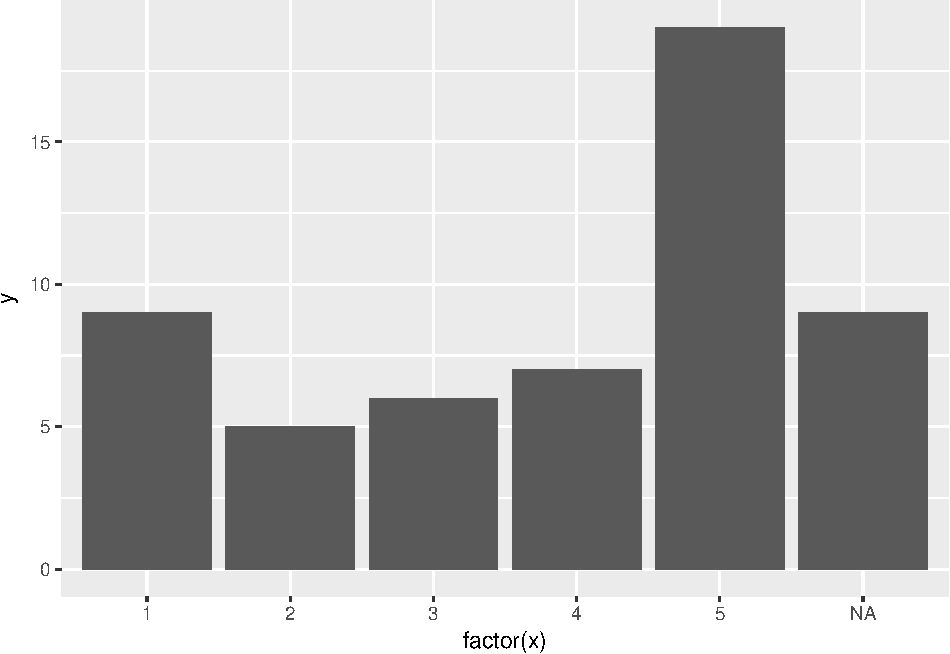
\includegraphics{jsm2017_files/figure-latex/unnamed-chunk-2-1.pdf}

\begin{Shaded}
\begin{Highlighting}[]
  \KeywordTok{ggplot}\NormalTok{(data_test,}
         \KeywordTok{aes}\NormalTok{(}\DataTypeTok{x =} \KeywordTok{factor}\NormalTok{(x),}
             \DataTypeTok{y =} \NormalTok{y)) +}\StringTok{ }
\StringTok{  }\KeywordTok{geom_boxplot}\NormalTok{()}
\end{Highlighting}
\end{Shaded}

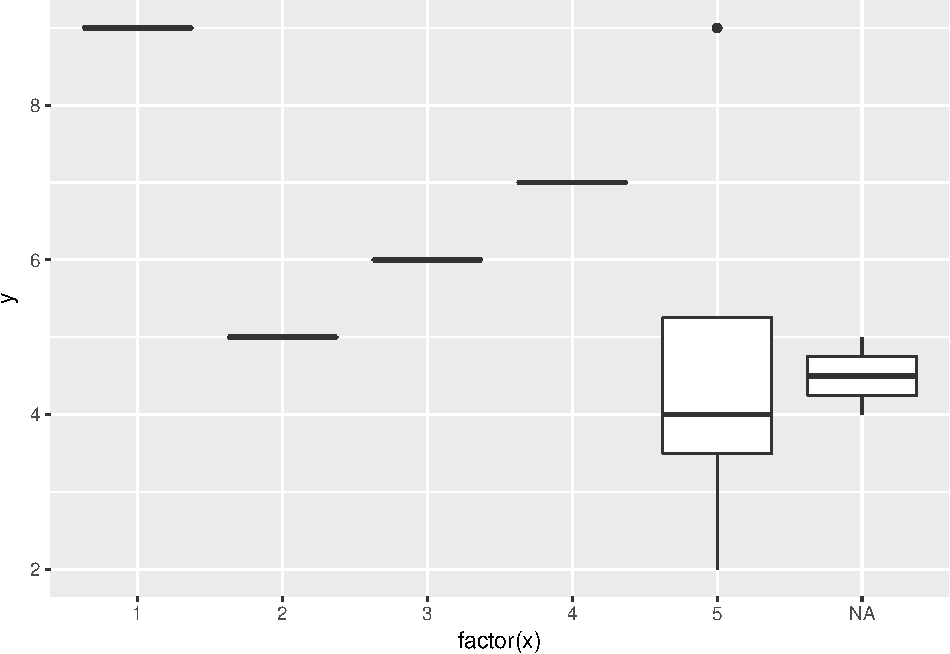
\includegraphics{jsm2017_files/figure-latex/unnamed-chunk-2-2.pdf}

\begin{Shaded}
\begin{Highlighting}[]
  \KeywordTok{ggplot}\NormalTok{(data_test,}
         \KeywordTok{aes}\NormalTok{(}\DataTypeTok{x =} \KeywordTok{factor}\NormalTok{(x),}
             \DataTypeTok{y =} \NormalTok{y)) +}\StringTok{ }
\StringTok{  }\KeywordTok{geom_point}\NormalTok{()}
\end{Highlighting}
\end{Shaded}

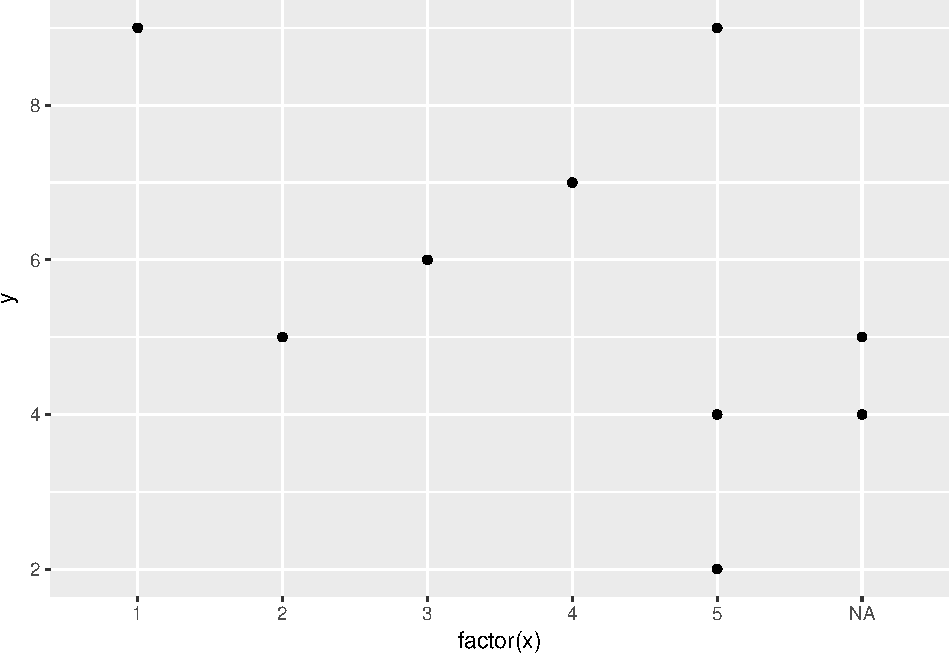
\includegraphics{jsm2017_files/figure-latex/unnamed-chunk-2-3.pdf}

\section{Data structures for missing
data}\label{data-structures-for-missing-data}

\begin{Shaded}
\begin{Highlighting}[]
\NormalTok{df_example <-}\StringTok{  }\NormalTok{tibble::}\KeywordTok{tribble}\NormalTok{(~V1, ~V2, ~V3, ~V4,}
                               \StringTok{"A"}\NormalTok{, }\DecValTok{15}\NormalTok{, }\FloatTok{1.2}\NormalTok{, }\OtherTok{NA}\NormalTok{,}
                               \StringTok{"A"}\NormalTok{, }\OtherTok{NA}\NormalTok{, }\OtherTok{NA}\NormalTok{, T,}
                               \StringTok{"A"}\NormalTok{, }\DecValTok{18}\NormalTok{, }\OtherTok{NA}\NormalTok{, F,}
                               \StringTok{"B"}\NormalTok{, }\DecValTok{5}\NormalTok{, }\FloatTok{1.6}\NormalTok{, T,}
                               \StringTok{"B"}\NormalTok{, }\OtherTok{NA}\NormalTok{, }\FloatTok{0.7}\NormalTok{, T,}
                               \StringTok{"B"}\NormalTok{, }\DecValTok{12}\NormalTok{, }\OtherTok{NA}\NormalTok{, F)}

\CommentTok{# df_example}

\KeywordTok{as_shadow}\NormalTok{(df_example)}
\end{Highlighting}
\end{Shaded}

\begin{verbatim}
## # A tibble: 6 × 4
##    V1_NA  V2_NA  V3_NA  V4_NA
##   <fctr> <fctr> <fctr> <fctr>
## 1    !NA    !NA    !NA     NA
## 2    !NA     NA     NA    !NA
## 3    !NA    !NA     NA    !NA
## 4    !NA    !NA    !NA    !NA
## 5    !NA     NA    !NA    !NA
## 6    !NA    !NA     NA    !NA
\end{verbatim}

\begin{Shaded}
\begin{Highlighting}[]
\KeywordTok{as_shadow}\NormalTok{(df_example) %>%}
\StringTok{  }\KeywordTok{mutate}\NormalTok{(}\DataTypeTok{rows =} \KeywordTok{row_number}\NormalTok{()) %>%}
\StringTok{  }\KeywordTok{gather}\NormalTok{(}\DataTypeTok{key =} \StringTok{"var"}\NormalTok{,}
         \DataTypeTok{value =} \StringTok{"miss"}\NormalTok{,}
         \NormalTok{-rows)}
\end{Highlighting}
\end{Shaded}

\begin{verbatim}
## # A tibble: 24 × 3
##     rows   var  miss
##    <int> <chr> <chr>
## 1      1 V1_NA   !NA
## 2      2 V1_NA   !NA
## 3      3 V1_NA   !NA
## 4      4 V1_NA   !NA
## 5      5 V1_NA   !NA
## 6      6 V1_NA   !NA
## 7      1 V2_NA   !NA
## 8      2 V2_NA    NA
## 9      3 V2_NA   !NA
## 10     4 V2_NA   !NA
## # ... with 14 more rows
\end{verbatim}

\begin{Shaded}
\begin{Highlighting}[]
\KeywordTok{bind_shadow}\NormalTok{(df_example)}
\end{Highlighting}
\end{Shaded}

\begin{verbatim}
## # A tibble: 6 × 8
##      V1    V2    V3    V4  V1_NA  V2_NA  V3_NA  V4_NA
##   <chr> <dbl> <dbl> <lgl> <fctr> <fctr> <fctr> <fctr>
## 1     A    15   1.2    NA    !NA    !NA    !NA     NA
## 2     A    NA    NA  TRUE    !NA     NA     NA    !NA
## 3     A    18    NA FALSE    !NA    !NA     NA    !NA
## 4     B     5   1.6  TRUE    !NA    !NA    !NA    !NA
## 5     B    NA   0.7  TRUE    !NA     NA    !NA    !NA
## 6     B    12    NA FALSE    !NA    !NA     NA    !NA
\end{verbatim}

Representing missing data structure is achieed using the shadow matrix,
introduced in Swayne and Buja {[}-@Swayne1998{]}. The shadow matrix is
the same dimension as the data, and consists of binary indicators of
``missingness'' of data values. In our case, missing is represented as
``NA'', and not missing is represented as ``!NA'', although these may be
represented as 1 and 0, repspectively. This helps us have a way to
describe the missingness structure explicitly. Representing it as its
own separate matrix also helps us separate out the multivariate nature
of missing data, as different cases have missing values in different
sets of variables.

the representation of the data where the missing values are regarded as
TRUE, and the present values are regarded as FALSE. To visualise this
matrix it is useful to gather the data into long form, going from each
row being an observation and each column being a variable, to columns.

It creates a tension as there is this extra dimension to the data.
Visualising missing data can be very challenging, and on the surface is
somewhat paradoxical: how do you visualise things that are missing? One
way to keep track of missing data is to consider a ``shadow matrix'', of
the data, where it is 1 if missing, and 0 is present. One can think of
the ``shadow matrix'' sitting under the actual data frame, like an
additional row sitting on the top.

One common method for visualising missing data is to display the data in
binary form of missing or not-missing. This approach can be very helpful
for giving an overview of which variables contain the most missingness,
and methods for rearranging the rows and columns (such as in the
seriation package), can be applied to find clusters, identifying other
interesting features of the data that may have previously been hidden or
unclear. This method has been used in other missing data packages such
as VIM, mi, Amelia, and MissingDataGUI.

XXX Start new section

\subsection{Visualisation of missing
data}\label{visualisation-of-missing-data}

Heatmap (plot of the long form

Facetted plots

Explain how the data structure facilitates these vis with ggplot2

Numerical summaries

You can also write a few sentences on computing on the fly vs data
storage

XXX End new section (this section incorporates/replaces things you've
got below)

XXX Start new section

\subsection{Usage}\label{usage}

Show a bunch of examples now, with some minimal R code

XXX End new section

These functions provide information on \ldots{} \ldots{} \ldots{}

\section{Data Structures}\label{data-structures}

\section{How the data structures facilitates the visualisation and the
summaries}\label{how-the-data-structures-facilitates-the-visualisation-and-the-summaries}

There are many methods for imputation such as \ldots{}

Mice provides imputation methods, diagnostics, and for user-written
imputation functions, among many other features.

We consider how numerical summaries and visualisation can be used to
explore missing data structure. In the future we would also like to
consider model based missing data structures.

Numerical summaries:

A good starting place for exploring missingness structure it to look at
numerical summaries. The \texttt{ggmissing} package provides functions
for summarising missing data, for example finding the overall proportion
of missing values in a dataset is obtained with
\texttt{percent\_missing\_df(data)}, in our case of using our dataset,
we find that 3.0061141\% of the data has missing values. similarly, we
can find the proportion of cases that contain a missing value with
\texttt{percent\_missing\_case}, giving 23.2336957\%, and the proportion
of variables that contain a missing value with
\texttt{percent\_missing\_var(tao)} = 37.5.

\begin{Shaded}
\begin{Highlighting}[]
\CommentTok{# percent_missing_df()}
\CommentTok{# miss_prop_df(tao)}
\CommentTok{# prop_na_df(tao)}
\CommentTok{# mean(is.na(tao))}

\NormalTok{prop_na <-}\StringTok{ }\NormalTok{function(x)\{}
  
  \NormalTok{prop_na_df <-}\StringTok{ }\KeywordTok{data_frame}\NormalTok{(}
    \DataTypeTok{df =} \KeywordTok{percent_missing_df}\NormalTok{(x),}
    \DataTypeTok{var =} \KeywordTok{percent_missing_var}\NormalTok{(x),}
    \DataTypeTok{case =} \KeywordTok{percent_missing_case}\NormalTok{(x)}
  \NormalTok{)}
  
  \NormalTok{prop_na_df}
  
\NormalTok{\}}

\KeywordTok{prop_na}\NormalTok{(airquality)}
\end{Highlighting}
\end{Shaded}

\begin{verbatim}
## # A tibble: 1 × 3
##         df      var     case
##      <dbl>    <dbl>    <dbl>
## 1 4.793028 33.33333 27.45098
\end{verbatim}

\begin{Shaded}
\begin{Highlighting}[]
\NormalTok{tao1 <-}\StringTok{ }\NormalTok{tao %>%}\StringTok{ }\KeywordTok{filter}\NormalTok{(year ==}\StringTok{ }\DecValTok{1997}\NormalTok{)}
\NormalTok{tao2 <-}\StringTok{ }\NormalTok{tao %>%}\StringTok{ }\KeywordTok{filter}\NormalTok{(year ==}\StringTok{ }\DecValTok{1993}\NormalTok{)}
\CommentTok{# }
\NormalTok{ggmissing::}\KeywordTok{summary_missing_var}\NormalTok{(tao)}
\end{Highlighting}
\end{Shaded}

\begin{verbatim}
## # A tibble: 8 × 3
##           variable n_missing    percent
##              <chr>     <int>      <dbl>
## 1         humidity        93 12.6358696
## 2         air.temp        81 11.0054348
## 3 sea.surface.temp         3  0.4076087
## 4             year         0  0.0000000
## 5         latitude         0  0.0000000
## 6        longitude         0  0.0000000
## 7            uwind         0  0.0000000
## 8            vwind         0  0.0000000
\end{verbatim}

\begin{Shaded}
\begin{Highlighting}[]
\NormalTok{ggmissing::}\KeywordTok{summary_missing_var}\NormalTok{(tao1)}
\end{Highlighting}
\end{Shaded}

\begin{verbatim}
## # A tibble: 8 × 3
##           variable n_missing  percent
##              <chr>     <int>    <dbl>
## 1         air.temp        77 20.92391
## 2             year         0  0.00000
## 3         latitude         0  0.00000
## 4        longitude         0  0.00000
## 5 sea.surface.temp         0  0.00000
## 6         humidity         0  0.00000
## 7            uwind         0  0.00000
## 8            vwind         0  0.00000
\end{verbatim}

\begin{Shaded}
\begin{Highlighting}[]
\NormalTok{ggmissing::}\KeywordTok{summary_missing_var}\NormalTok{(tao2)}
\end{Highlighting}
\end{Shaded}

\begin{verbatim}
## # A tibble: 8 × 3
##           variable n_missing    percent
##              <chr>     <int>      <dbl>
## 1         humidity        93 25.2717391
## 2         air.temp         4  1.0869565
## 3 sea.surface.temp         3  0.8152174
## 4             year         0  0.0000000
## 5         latitude         0  0.0000000
## 6        longitude         0  0.0000000
## 7            uwind         0  0.0000000
## 8            vwind         0  0.0000000
\end{verbatim}

\begin{Shaded}
\begin{Highlighting}[]
\CommentTok{# }
\end{Highlighting}
\end{Shaded}

\textbf{from here}

\begin{itemize}
\tightlist
\item
  finish the summary methods
\item
  finish the visualisation methods possible
\item
  read and write again
\item
  write down a list of things that I need to fix with ggmissing etc.
\end{itemize}

Conditional summaries, or summaries grouped by another variable.

summary windows present - \% of values that are missing - \% of
varaibles containing missings - the percent of cases that have at least
one missing value - tabulation of the number of values missing per case.

This study is taken from the R package norm, and MissingDataGUI

it would be really cool if we could implement dplyr \texttt{group\_by}
syntax for the data, to produce summaries of missingness for 1993 and
1997 respectively.

Numerical summaries can occur at a few different levels

Single number summaries:

\begin{itemize}
\tightlist
\item
  The proportion elements in dataset that contains missing values
\item
  The proportion of variables that contain any missing values
\item
  the proportion of cases that contain any missing values
\end{itemize}

tabular summaries: - The proportion of missings in every column
(variable) - the proportion of missings in every row (case)

further summaries that use more steps: table\_missing\_case(airquality)
table\_missing\_var(airquality)

sumamries that return dataframes:

\begin{Shaded}
\begin{Highlighting}[]
\KeywordTok{summary_missing_var}\NormalTok{(airquality)}
\end{Highlighting}
\end{Shaded}

\begin{verbatim}
## # A tibble: 6 × 3
##   variable n_missing   percent
##      <chr>     <int>     <dbl>
## 1    Ozone        37 24.183007
## 2  Solar.R         7  4.575163
## 3     Wind         0  0.000000
## 4     Temp         0  0.000000
## 5    Month         0  0.000000
## 6      Day         0  0.000000
\end{verbatim}

\begin{Shaded}
\begin{Highlighting}[]
\KeywordTok{summary_missing_case}\NormalTok{(airquality)}
\end{Highlighting}
\end{Shaded}

\begin{verbatim}
## # A tibble: 153 × 3
##     case n_missing  percent
##    <int>     <int>    <dbl>
## 1      1         0  0.00000
## 2      2         0  0.00000
## 3      3         0  0.00000
## 4      4         0  0.00000
## 5      5         2 33.33333
## 6      6         1 16.66667
## 7      7         0  0.00000
## 8      8         0  0.00000
## 9      9         0  0.00000
## 10    10         1 16.66667
## # ... with 143 more rows
\end{verbatim}

Visual summaries:

Exploring missingness

exploring missinginess in multivariate - geom\_missing\_point()

naniar helps open the door to a crazy world where there are tools to
handle missings (NAs).

The aim of naniar is to:

\begin{itemize}
\tightlist
\item
  facilitate the visualisation of missing data
\item
  exploration of possible causes for missing data
\item
  modelling possible mechanisms for missing data
\item
  exploring missing data imputation methods.
\end{itemize}

\begin{enumerate}
\def\labelenumi{\arabic{enumi}.}
\tightlist
\item
  Exploring missing data
\item
  Visualising missing data
\item
  Modelling mechanisms for missing data
\item
  Testing mechanisms for missing data
\item
  Confirming mechanisms for missing data
\end{enumerate}

\begin{itemize}
\tightlist
\item
  Helpers for working with missing data
\item
  Systematic principles for exploring missing data
\item
  Guidance on how to sensibly impute missing data
\item
  Visualisation of missing data imputation
\end{itemize}

Exploration - vis\_miss - sort\_cols - cluster Visualisations - Model
missing cluster - relate clusters to missing data mechanism -
testing/modelling - somehow relate this cluster to missing data
mechanism - m-fold, or mcmc)

It is important to remember that there isn't a ``solution'' to the
missing data problem, but that instead there are much better ways of
doing missing data analysis.

smaller tasks: - Visualise whole data frames + missingness: visdat -
Exploratory graphics for missing data: ggmissing, Geoms, - Model
missingness structure: - Decision tree method + hierarchical clustering
- Use missingness structure to infer patterns / impute:

\texttt{nainr} \texttt{narniar} \texttt{narnia}: A package to a world
where missing data makes more sense.

Other potential names, for historical reasons: \texttt{banana}:
\texttt{narwhal} \texttt{nagpie} \texttt{nagpipes} \texttt{naan}\\
\texttt{nacho}\\
\texttt{nada} \texttt{nana} \texttt{misstletoe} \texttt{natrix}

Other commands that might be useful? \texttt{is\_na} \texttt{fill\_na}
\texttt{drop\_na} \texttt{is\_null}

note on the use of the ``upsidedown''/shadowmatrix having its own
missing values, where we go from being MISSING / !MISSING to MISSING /
MISSING\_REASON\_\#1 / MISSING\_REASON\_\#2 / etc.. - this idea of a
``senteinel value'', which I read about in this
\href{blog\%20post}{http://www.residentmar.io/2016/06/12/null-and-missing-data-python.html}
\textgreater{} \ldots{}a sentinel value, a special bit pattern in the
data column's native type flagging a missing value. This is a
traditional way of indicating missing data---recording unknown income as
-99 or an unknown year as 0, for example---which is used in-place
(hopefully with documentation!) by many datasets.The trouble is that
sentinal values are in no way durable. -99 could be a valid year and 0
could be a valid income! Without a special reserved keyword, a sentinel
robs you of a value that you might otherwise want to use. They have to
be considered on a case-by-case, column-by-column basis, a burdensome
thing.

Sometimes just working out where to start can be difficult and even
paralysing.

\section{Defining missing data and its various
forms.}\label{defining-missing-data-and-its-various-forms.}

It is helpful to first define what missing data is, and what it is not.
Missing data is data that we know should exist, but for some particular
reason is not recorded. For example, if there is temperature data
recorded every hour of every day, and one particular hour is missing on
a particular day, this is missing data. This is contrasted to data that
does not exist at all, for example, combining person-level data with
environment level data - A person would not have an ambient temperature,
and an environment does not have a pulse. These data are sometimes
referred to as NULL data, or non-data.

One of the motivations for understanding structure of missing data is to
understand \emph{why} it is missing in the first place. In the example
above for the temperature data, the temperature might not have been
recorded due to instrument failure, or system-wide shut down, perhaps it
was scheduled for maintenance.

While humans are very good at finding patterns, a model-driven approach
provides a more precise and potentially more automatic framework for
exploring missing data. We propose the use of decision trees as a
complementary tool for doing this.

Interesting, potentially incorrect blog post about this:

This means that when answering the question ``is this data entry
filled?'' one must actually consider three possible answers: ``Yes'',
``No, but it can be'', and ``No, and it cannot be''.

mice features:

\begin{itemize}
\tightlist
\item
  Columnwise specification of the imputation model
\item
  Support for arbitrary patterns of missing data
\item
  Passive imputation techniques that maintain consistency among data
  transformations
\item
  Subset selection of predictors
\item
  Support of arbitrary complete-data methods
\item
  Support pooling various types of statistics
\item
  Diagnostics for imputations
\item
  Callable user-written imputation functions
\end{itemize}

\section{Extras}\label{extras}

\subsection{Previous examples of missing
data}\label{previous-examples-of-missing-data}

For example, assessments of lung function taken at a workplace may be
missing for workers who are on vacation. If there is no known or
measurable relationship between the timing of the tests and the timing
of vacations, and if the other relevant features of the workers who are
on vacation at the time of the tests are similar to that of other
workers, then these missing data can be considered MCAR.

For example if the missing lung function data occurs in workers who are
being assessed for depression, and if there is no relationship between
lung function and depression, then it can be considered as MAR. For
example, if BMI is of interest, but those with especially large BMIs are
more likely to have missing BMI data, these data can be considered as
MNAR. It is important for researchers to recognise MNAR as it introduces
bias into the estimation of associations and parameters of interest. For
example, if lung function and BMI are negatively correlated, an estimate
of BMI based on the MNAR may be too low.

These three varieties of missing data could be further divided into a
knowable structure (MAR) or an unknown structure (MAR or MNAR), where
the process driving data becoming missing are either known or unknown,
and structure refers to variables and interactions that may influence
missingness. Data MCAR are without a missingness structure, as
missingness does not have any dependence on other variables. Determining
whether this is known or unknown is important for determining whether
bias may be introduced into the analysis.

\subsection{on tests for missing data}\label{on-tests-for-missing-data}

Tests confirming whether data is MCAR or not are very useful as they
open up the doors for the use of standard multiple imputation
techniques. As described by Little,who proposed a single test statistic
for testing MCAR, involving an evaluation of equality of means between
identified missing data groups. Rejection of this test result gives
strong evidence that the data are not MCAR. Little's test of MCAR is
widely used today, especially in social science8 and medical research.9
Recent research has also provided statistical tests and software that
evaluate missing data via patterns, equality of means, and homogeneity
of variance, and allow for non-normal data.

This is achieved, for example, in the MissMech package for the R
statistical software,10 which uses imputation (from either normal or
non-normal distributions) to compare means and covariances. These tests
enable the researcher to determine whether or not there is sufficient
evidence for data to be declared as MCAR.

However, understanding how and why missingness is being generated can
become arduous when handling larger data sets, as they can have many
missingness patterns, making inference difficult, as there are many
combinations of missingness to explore. Reliance on statistical
significance testing to assess whether data are missing may fail to
address settings where there may not be significant missingness, but a
complete case analysis may still result in bias (11). Approaches that
elucidate missingness structure that are simple to understand and
implement, are therefore still in demand.

\subsection{on other methods for missing
data}\label{on-other-methods-for-missing-data}

Common methods of handling missing data, such as complete case analysis,
missing indicator method, and last case carried forward have been shown
to be acceptable when data is MCAR.12 ,13 That being said, most
recommendations now are to use multiple imputation, but subject to some
care as it only reduces bias from analysis when data are MAR or MCAR;
multiple imputation also requires variables that influence missingness
to be included in the imputation model.1--4 ,14 When data are MNAR,
multiple imputation can be used but requires the MNAR mechanism to be
known, which is not often undertaken in practice.3 Improving the
understanding of missingness structure in a data set allows for
consideration of other appropriate multiple imputation methods, or other
methods to incorporate partially observed variables, such as random
effect models, Bayesian methods, down-weighting analyses, or pattern
mixture models.2 ,15 ,16


\end{document}
